\documentclass[11pt, a4paper]{article}

% --- Preamble ---
\usepackage[utf8]{inputenc} % Allows inputting UTF-8 characters
\usepackage[T1]{fontenc}    % Optimizes font encoding
\usepackage[english]{babel} % Language settings
\usepackage[margin=1in]{geometry} % Page margins
\usepackage{amsmath, amssymb} % For mathematical symbols and equations
\usepackage{graphicx}       % For including images
\graphicspath{{media/}}     % Tells LaTeX where to look for images
\usepackage{hyperref}       % For clickable links in the PDF (e.g., table of contents)
\hypersetup{
    colorlinks=true,
    linkcolor=blue,
    filecolor=magenta,
    urlcolor=cyan,
    pdftitle={Discrete Mathematics Project Report: Graph Theory and Graph Coloring},
    pdfauthor={Your Name},
    pdfsubject={Graph Theory, Graph Coloring, Discrete Mathematics},
    pdfkeywords={Graph, Coloring, Chromatic Number, Applications, TikZ, Algorithms},
}
\usepackage{fancyhdr}       % For custom headers/footers
\usepackage{enumitem}       % For customizing list environments
\usepackage{setspace}       % For setting line spacing
\usepackage{tikz}           % For drawing diagrams
\usetikzlibrary{graphs, graphs.standard, arrows, positioning, fit, shapes, patterns} % TikZ libraries for convenience

% Define colors for graph coloring examples
\definecolor{color1}{RGB}{255,105,97} % Reddish
\definecolor{color2}{RGB}{119,221,119} % Greenish
\definecolor{color3}{RGB}{174,198,207} % Bluish-grey
\definecolor{color4}{RGB}{255,255,153} % Yellowish

% Custom header/footer setup
% Define a custom pagestyle for the main content pages
\fancypagestyle{reportstyle}{
    \fancyhf{} % Clear all headers/footers
    \fancyhead[L]{Discrete Maths Project}
    % Place the header image on the right side. Adjust height as needed.
    \fancyhead[R]{
\includegraphics[height=0.7cm]{header.png}}
    \fancyfoot[C]{\thepage}
    \renewcommand{\headrulewidth}{0.4pt}
    \renewcommand{\footrulewidth}{0.4pt}
}

% Line spacing
\onehalfspacing % 1.5 line spacing

% --- Title Page Information ---
\title{
    \vspace{-2cm} % Adjust vertical space if needed, if logo is too high
    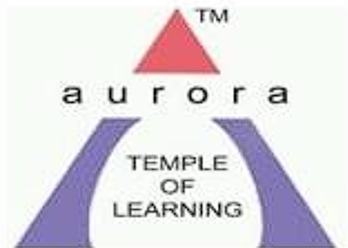
\includegraphics[width=0.4\textwidth]{aurora_logo.png} \\ % Logo on the title page
    \vspace{1cm} % Space between logo and title
    \textbf{Project Report on Graph Theory and Graph Coloring}
}
\author{
    \textbf{Your Name} \\
    Student ID: \texttt{XXXXXXXX} \\
    Department of \textit{Your Department} \\
    \textit{Your University}
}
\date{\today} % Or specify a date like \date{October 26, 2023}

% --- Document Start ---
\begin{document}

\maketitle % Displays the title page

\thispagestyle{empty} % No page number on the title page for the title page itself
\newpage

% Apply the custom pagestyle for the rest of the document starting from Abstract
\pagestyle{reportstyle}

% --- Abstract ---
\begin{abstract}
This report delves into the fascinating world of Graph Theory, a fundamental area of Discrete Mathematics, with a particular focus on Graph Coloring. We begin by introducing the basic definitions and concepts of graphs, including vertices, edges, and various types of graphs, and exploring various graph representations. Following this, the core principles of graph coloring are explored in detail, defining concepts such as chromatic number for vertex, edge, and face coloring, and discussing common algorithms like the greedy coloring algorithm and more sophisticated exact and approximate approaches. The report highlights diverse and critical applications of graph coloring in real-world scenarios, ranging from scheduling and resource allocation to map coloring, register allocation in compilers, and network design, illustrating these concepts with \texttt{TikZ} diagrams. Finally, a conclusion summarizes the key findings and emphasizes the pervasive importance of graph theory and its coloring techniques in solving complex problems across different scientific and engineering disciplines.
\end{abstract}

\newpage
\tableofcontents % Generates the table of contents
\newpage

% --- Introduction ---
\section{Introduction}
Graph Theory, a vibrant and extensively studied branch of discrete mathematics, provides a powerful and intuitive framework for modeling and analyzing relationships between objects. At its core, a graph consists of a set of vertices (or nodes) and a set of edges (or links) connecting pairs of these vertices. Its genesis is often attributed to Leonhard Euler's solution to the Königsberg Bridge Problem in 1736, a puzzle that elegantly demonstrated the utility of abstracting physical layouts into a network of nodes and connections. Since then, graph theory has evolved into an indispensable analytical and problem-solving tool, permeating diverse fields such as computer science, electrical engineering, operations research, social sciences, biology, and chemistry. Its ability to represent complex structures, from social networks to computer circuits, makes it a cornerstone of modern scientific inquiry.

This report aims to provide a comprehensive overview of fundamental graph theory concepts, laying the groundwork for a detailed discussion of graph coloring. Graph coloring, a specialized form of graph labeling, involves assigning labels (often referred to as "colors") to elements of a graph (vertices, edges, or faces) subject to specific constraints. The elegance of graph coloring lies in its profound ability to model and solve a myriad of complex resource allocation, scheduling, and conflict resolution problems. By exploring the formal definitions, key algorithms (both heuristic and exact), and a wide array of practical applications, this report will demonstrate the significant role graph coloring plays in addressing real-world challenges across various disciplines, supplemented with illustrative \texttt{TikZ} diagrams for clarity.

% --- Fundamentals of Graph Theory ---
\section{Fundamentals of Graph Theory}
A graph $G$ is formally defined as an ordered pair $(V, E)$, where $V$ is a finite, non-empty set of vertices (or nodes), and $E$ is a set of edges (or links) that connect pairs of vertices from $V$. The nature of these connections defines the type of graph.

\subsection{Basic Definitions and Terminology}
\begin{itemize}[noitemsep,topsep=3pt,parsep=3pt,partopsep=0pt]
    \item \textbf{Vertex (Node)}: A fundamental entity or point in a graph. Represented as a circle or point, it can signify an object, location, person, or any discrete item.
    \item \textbf{Edge (Link/Arc)}: A connection between two vertices. An edge $(u,v)$ or $uv$ signifies a relationship or interaction between vertex $u$ and vertex $v$. Edges can be lines or curves.
    \item \textbf{Adjacent Vertices}: Two vertices are adjacent if they are connected by an edge.
    \item \textbf{Incident Edge}: An edge $e$ is incident to a vertex $v$ if $v$ is one of the endpoints of $e$.
    \item \textbf{Degree of a Vertex ($\deg(v)$)}: The number of edges incident to a vertex $v$. For directed graphs, we distinguish between in-degree (number of edges pointing to $v$) and out-degree (number of edges pointing from $v$). The sum of degrees of all vertices in any graph is twice the number of edges.
    \item \textbf{Path}: A sequence of distinct vertices $v_0, v_1, \ldots, v_k$ such that $v_i$ and $v_{i+1}$ are adjacent for all $0 \le i < k$. The length of a path is the number of edges it contains ($k$).
    \item \textbf{Cycle}: A closed path that starts and ends at the same vertex, with all intermediate vertices being distinct. The length of a cycle is its number of edges.
    \item \textbf{Simple Graph}: A graph that contains no loops (an edge connecting a vertex to itself) and no multiple edges (more than one edge between the same pair of vertices). Unless explicitly stated otherwise, "graph" in the context of coloring usually refers to a simple graph.
\end{itemize}

\subsection{Types of Graphs}
Graphs can be classified based on the properties of their edges, vertices, and overall structure:
\begin{itemize}[noitemsep,topsep=3pt,parsep=3pt,partopsep=0pt]
    \item \textbf{Undirected Graph}: Edges have no direction. If $(u,v)$ is an edge, it implies a symmetric relationship; the connection from $u$ to $v$ is the same as from $v$ to $u$.
    \item \textbf{Directed Graph (Digraph)}: Edges have a specific direction, typically indicated by an arrow. An edge $(u,v)$ means there is a connection from $u$ to $v$, but not necessarily from $v$ to $u$. This is useful for modeling workflows or causal relationships.
    \item \textbf{Weighted Graph}: Each edge or vertex has an associated numerical value, or "weight," which can represent distance, cost, capacity, time, or strength of connection.
    \item \textbf{Complete Graph ($K_n$)}: A simple undirected graph where every pair of distinct vertices is connected by a unique edge. A complete graph with $n$ vertices is denoted $K_n$.
    \item \textbf{Bipartite Graph}: A graph whose vertices can be divided into two disjoint and independent sets, $U$ and $V$, such that every edge connects a vertex in $U$ to one in $V$. There are no edges within $U$ or within $V$.
    \item \textbf{Planar Graph}: A graph that can be drawn on a plane (or a sphere) such that no edges cross each other except at their common vertices. These graphs are particularly important in map coloring.
    \item \textbf{Tree}: A connected undirected graph that contains no simple cycles. Trees are fundamental in computer science for data structures (e.g., binary search trees), network topology, and hierarchical organization.
    \item \textbf{Subgraph}: A graph $H=(V', E')$ is a subgraph of $G=(V, E)$ if $V' \subseteq V$ and $E' \subseteq E$. If $H$ contains all edges of $G$ that connect vertices in $V'$, then $H$ is an induced subgraph.
\end{itemize}

\begin{figure}[h!]
    \centering
    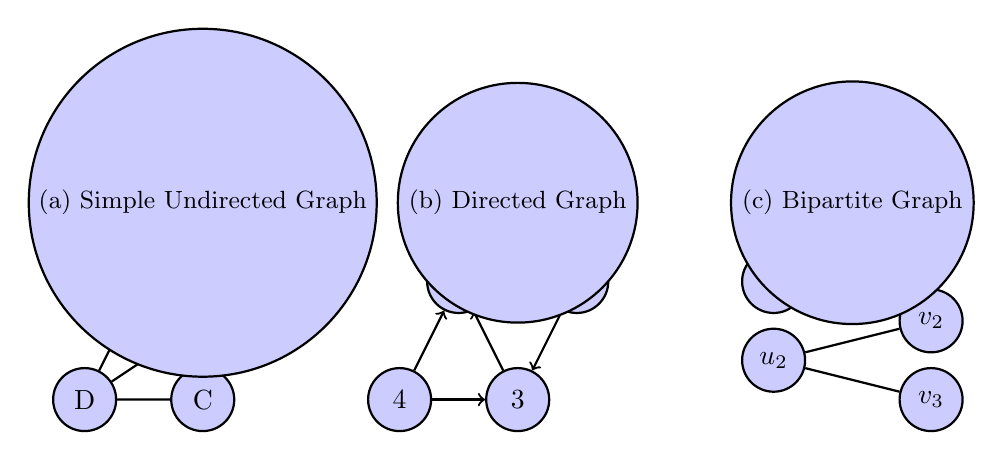
\begin{tikzpicture}[%
        node distance=1.5cm,
        every node/.style={circle, draw, fill=blue!20, minimum size=0.8cm},
        thick,
        % Global options for graphs
        graphs/every graph/.style={
            nodes={circle, draw, fill=blue!20, minimum size=0.8cm},
            edges={thick}
        }
    ]
    % --- Simple Graph ---
    \begin{scope}[xshift=0cm]
        \node (A) at (0,0) {A};
        \node (B) at (1.5,0) {B};
        \node (C) at (0.75,-1.5) {C};
        \node (D) at (-0.75,-1.5) {D};

        \draw (A) -- (B) -- (C) -- (D) -- (A) -- (C);
        \path (B) edge (D);
        \node at (0.75, 1) {\small (a) Simple Undirected Graph};
    \end{scope}

    % --- Directed Graph ---
    \begin{scope}[xshift=4cm]
        \node (1) at (0,0) {1};
        \node (2) at (1.5,0) {2};
        \node (3) at (0.75,-1.5) {3};
        \node (4) at (-0.75,-1.5) {4};

        \draw[->] (1) -- (2);
        \draw[->] (2) -- (3);
        \draw[->] (3) -- (1);
        \draw[->] (4) -- (1);
        \draw[->] (4) -- (3);
        \node at (0.75, 1) {\small (b) Directed Graph};
    \end{scope}

    % --- Bipartite Graph ---
    \begin{scope}[xshift=8cm]
        \node (u1) at (0,0) {$u_1$};
        \node (u2) at (0,-1) {$u_2$};
        \node (v1) at (2,0.5) {$v_1$};
        \node (v2) at (2,-0.5) {$v_2$};
        \node (v3) at (2,-1.5) {$v_3$};

        \draw (u1) -- (v1);
        \draw (u1) -- (v2);
        \draw (u2) -- (v2);
        \draw (u2) -- (v3);
        \node at (1, 1) {\small (c) Bipartite Graph};
    \end{scope}
    \end{tikzpicture}
    \caption{Examples of different types of graphs drawn with \texttt{TikZ}: (a) a simple undirected graph, (b) a directed graph, and (c) a bipartite graph with partition sets $\{u_1, u_2\}$ and $\{v_1, v_2, v_3\}$.}
    \label{fig:tikz_graph_types}
\end{figure}

\subsection{Graph Connectivity and Paths}
Connectivity is a crucial property of graphs, defining how well-interconnected its vertices are.
\begin{itemize}[noitemsep,topsep=3pt,parsep=3pt,partopsep=0pt]
    \item \textbf{Connected Graph}: An undirected graph is connected if there is at least one path between every pair of distinct vertices. If a graph is not connected, it is called disconnected.
    \item \textbf{Connected Components}: A connected component of an undirected graph is a subgraph in which any two vertices are connected to each other by paths, and which is connected to no additional vertices in the supergraph. A disconnected graph consists of multiple connected components.
    \item \textbf{Bridge (Cut Edge)}: An edge whose removal increases the number of connected components of the graph. Bridges are critical for graph robustness.
    \item \textbf{Articulation Point (Cut Vertex)}: A vertex whose removal (along with all incident edges) increases the number of connected components of the graph. Articulation points represent single points of failure in a network.
\end{itemize}

\subsection{Graph Representations}
For computational tasks, graphs need to be stored efficiently in memory. The choice of representation often depends on the graph's density (number of edges relative to maximum possible edges) and the specific operations to be performed.
\begin{itemize}[noitemsep,topsep=3pt,parsep=3pt,partopsep=0pt]
    \item \textbf{Adjacency Matrix}: An $N \times N$ matrix (where $N$ is the number of vertices) where $A_{ij}=1$ if there is an edge between vertex $i$ and vertex $j$, and $A_{ij}=0$ otherwise. For weighted graphs, $A_{ij}$ stores the weight. This representation is space-inefficient for sparse graphs ($O(N^2)$ space) but allows for $O(1)$ lookup to check if an edge exists.
    \item \textbf{Adjacency List}: An array of lists (or linked lists). For each vertex $i$, the list at index $i$ contains all vertices adjacent to $i$. This is more space-efficient for sparse graphs ($O(N+M)$ space, where $M$ is the number of edges) and efficient for iterating over neighbors of a vertex.
\end{itemize}

\section{Graph Coloring}
Graph coloring, in its most common form, refers to vertex coloring, but it also extends to edges and faces. The general problem involves assigning labels (colors) to graph elements such that adjacent or related elements have different colors, aiming to minimize the total number of colors used.

\subsection{Vertex Coloring}
Vertex coloring is an assignment of colors to the vertices of a graph $G=(V, E)$ such that no two adjacent vertices share the same color. This is known as a \textit{proper coloring}.

\begin{itemize}[noitemsep,topsep=3pt,parsep=3pt,partopsep=0pt]
    \item \textbf{Proper Coloring}: A function $c: V \to \{1, 2, \ldots, k\}$ such that for every edge $(u,v) \in E$, it holds that $c(u) \neq c(v)$. The value $k$ is the number of colors used.
    \item \textbf{Chromatic Number ($\chi(G)$)}: The minimum number of colors required for a proper vertex coloring of a graph $G$. A graph $G$ is $k$-colorable if its chromatic number is less than or equal to $k$. Finding the chromatic number is one of the central problems in graph theory.
\end{itemize}

\subsubsection{Properties and Bounds of Chromatic Number}
The chromatic number is a fundamental graph invariant with several interesting properties and established bounds:
\begin{itemize}[noitemsep,topsep=3pt,parsep=3pt,partopsep=0pt]
    \item \textbf{Clique Number ($\omega(G)$)}: A clique in a graph is a subgraph that is complete. The clique number $\omega(G)$ is the number of vertices in the largest clique of $G$. If $G$ contains $K_n$ as a subgraph, then at least $n$ distinct colors are required, as all vertices in a clique must have different colors. Thus, a fundamental lower bound is $\chi(G) \ge \omega(G)$.
    \item \textbf{Upper Bound based on Maximum Degree ($\Delta(G)$)}: The maximum degree $\Delta(G)$ of a graph $G$ is the largest degree of any vertex in $G$. A simple upper bound is $\chi(G) \le \Delta(G) + 1$. This can be achieved by a greedy algorithm.
    \item \textbf{Brooks' Theorem}: This theorem provides a tighter upper bound. It states that for any connected graph $G$ that is not a complete graph or an odd cycle, $\chi(G) \le \Delta(G)$. For complete graphs $K_n$, $\chi(K_n)=n=\Delta(K_n)+1$. For odd cycles $C_{2k+1}$, $\chi(C_{2k+1})=3=\Delta(C_{2k+1})+1$.
    \item \textbf{Nordhaus-Gaddum Theorem}: This theorem relates the chromatic number of a graph $G$ to that of its complement graph $\bar{G}$ (a graph with the same vertices as $G$, but edges connect exactly those pairs of vertices not connected in $G$). It states: $\chi(G) + \chi(\bar{G}) \le n+1$ and $\chi(G) \cdot \chi(\bar{G}) \ge n$, where $n$ is the number of vertices in $G$.
\end{itemize}

\begin{figure}[h!]
    \centering
    \begin{tikzpicture}[%
        node distance=1.5cm,
        every node/.style={circle, draw, minimum size=0.8cm},
        thick
    ]
    % --- Uncolored Graph ---
    \begin{scope}[xshift=0cm]
        \node (A) at (0,0) {A};
        \node (B) at (1.5,0) {B};
        \node (C) at (0.75,-1.5) {C};
        \node (D) at (-0.75,-1.5) {D};
        \node (E) at (-1.5,0) {E};

        \draw (A) -- (B) -- (C) -- (D) -- (A) -- (E);
        \path (B) edge (D);
        \path (E) edge (D);
        \node at (0, 1) {\small (a) Uncolored Graph};
    \end{scope}

    % --- Properly Colored Graph ---
    \begin{scope}[xshift=5cm]
        \node[fill=color1] (A) at (0,0) {A};
        \node[fill=color2] (B) at (1.5,0) {B};
        \node[fill=color3] (C) at (0.75,-1.5) {C};
        \node[fill=color2] (D) at (-0.75,-1.5) {D};
        \node[fill=color1] (E) at (-1.5,0) {E};

        \draw (A) -- (B) -- (C) -- (D) -- (A) -- (E);
        \path (B) edge (D);
        \path (E) edge (D);
        \node at (0, 1) {\small (b) Proper Vertex Coloring ($\chi(G)=3$)};
        % Color legend
        \node[color1, fill=color1, draw=black] at (2.5, 0.5) {}; \node[right=0.2cm of color1.east, font=\tiny] {Color 1};
        \node[color2, fill=color2, draw=black] at (2.5, 0) {}; \node[right=0.2cm of color2.east, font=\tiny] {Color 2};
        \node[color3, fill=color3, draw=black] at (2.5, -0.5) {}; \node[right=0.2cm of color3.east, font=\tiny] {Color 3};
    \end{scope}
    \end{tikzpicture}
    \caption{Example of vertex coloring: (a) An uncolored graph. (b) A proper 3-coloring of the graph, demonstrating its chromatic number is 3 (as A and E can share Color 1, and B and D can share Color 2, with C needing a unique Color 3).}
    \label{fig:tikz_vertex_coloring}
\end{figure}

\subsection{Edge Coloring}
Edge coloring is an assignment of colors to the edges of a graph such that no two edges incident to the same vertex share the same color. This means all edges meeting at a common vertex must have distinct colors. The minimum number of colors required for a proper edge coloring is called the \textbf{chromatic index}, denoted $\chi'(G)$.
\begin{itemize}[noitemsep,topsep=3pt,parsep=3pt,partopsep=0pt]
    \item \textbf{Vizing's Theorem}: This important theorem states that for any simple graph $G$, its chromatic index $\chi'(G)$ is either equal to the maximum degree of the graph, $\Delta(G)$, or one more than the maximum degree, i.e., $\chi'(G) = \Delta(G)$ or $\chi'(G) = \Delta(G)+1$. Graphs with $\chi'(G) = \Delta(G)$ are called Class 1, and those with $\chi'(G) = \Delta(G)+1$ are called Class 2.
\end{itemize}

\subsection{Face Coloring}
Face coloring applies specifically to planar graphs, which are graphs that can be drawn on a plane without any edges crossing. In face coloring, regions (faces) bounded by edges are colored. The constraint is that adjacent faces (sharing a common edge) must have different colors.
\begin{itemize}[noitemsep,topsep=3pt,parsep=3pt,partopsep=0pt]
    \item \textbf{Four Color Theorem}: One of the most famous and historically significant theorems in graph theory, it states that any planar graph (or map) can be face-colored using at most four colors. This theorem was famously proven with the aid of computers by Kenneth Appel and Wolfgang Haken in 1976, marking a significant milestone in computational mathematics.
\end{itemize}

\subsection{Algorithms for Graph Coloring}
Finding the chromatic number $\chi(G)$ of a general graph $G$ is an NP-hard problem, implying that no efficient (polynomial-time) algorithm is known that can guarantee an optimal solution for all graphs. This computational complexity necessitates the use of different approaches: exact algorithms for smaller instances or specific graph types, and heuristic/approximation algorithms for larger, more complex graphs where optimality is less critical than speed.

\subsubsection{Exact Algorithms (for Optimal Coloring)}
These algorithms are designed to find the true chromatic number $\chi(G)$ and an optimal coloring, but their computational cost grows exponentially with the size of the graph.
\begin{itemize}[noitemsep,topsep=3pt,parsep=3pt,partopsep=0pt]
    \item \textbf{Brute-Force/Backtracking}: This approach systematically explores all possible color assignments. It's often implemented recursively: it tries to color one vertex at a time with the minimum possible color. If a proper coloring cannot be extended from the current choices (e.g., a neighbor already has the chosen color), it "backtracks" and tries a different color. This method is guaranteed to find an optimal coloring but is extremely slow for all but very small graphs.
    \item \textbf{Integer Linear Programming (ILP) Formulation}: Graph coloring can be formulated as an Integer Linear Programming problem. This involves defining binary variables $x_{v,c}$ (where $x_{v,c}=1$ if vertex $v$ gets color $c$, and $0$ otherwise) and minimizing the total number of colors used, subject to constraints. The constraints ensure that each vertex gets exactly one color and that adjacent vertices always receive different colors. ILP solvers can find optimal solutions but can be very time-consuming.
    \item \textbf{Branch and Bound}: An optimization technique applied to backtracking search. It prunes branches of the search tree that are guaranteed not to lead to an optimal solution, typically by maintaining a lower bound on the optimal number of colors. If a partial coloring already uses more colors than a known upper bound, that branch is discarded.
\end{itemize}

\subsubsection{Heuristic and Approximation Algorithms}
Given the NP-hardness of finding an optimal coloring, for many practical applications, an approximation (a coloring that is "good enough" but not necessarily minimal) is acceptable if it can be found efficiently.
\begin{itemize}[noitemsep,topsep=3pt,parsep=3pt,partopsep=0pt]
    \item \textbf{Greedy Coloring Algorithm}: This is the simplest and most widely used heuristic due to its ease of implementation and speed.
    \begin{enumerate}[label=(\roman*),noitemsep,topsep=3pt,parsep=3pt,partopsep=0pt]
        \item Establish an order for the vertices of the graph $V = \{v_1, v_2, \ldots, v_n\}$. This ordering can be arbitrary, or based on properties like vertex degree.
        \item Assign the first vertex ($v_1$) the smallest available color (conventionally, color 1).
        \item For each subsequent vertex $v_i$ (from $i=2$ to $n$), assign it the smallest positive integer color that has not been used by any of its already-colored neighbors.
    \end{enumerate}
    The number of colors used by a greedy algorithm depends heavily on the initial ordering of vertices. It does not guarantee an optimal coloring, but it is fast ($O(N+M)$ in general).
    \item \textbf{Welsh-Powell Algorithm}: A specific variant of greedy coloring that often performs better. Vertices are ordered in decreasing order of their degrees (highest degree first) before applying the standard greedy coloring procedure. This strategy aims to color the most constrained vertices early, potentially reducing the total number of colors needed.
    \item \textbf{DSatur Algorithm}: A more sophisticated greedy-like algorithm that prioritizes coloring vertices with the highest "saturation degree." The saturation degree of a vertex is defined as the number of different colors already used by its neighbors. If ties occur (multiple vertices have the same highest saturation degree), the algorithm breaks them by choosing the vertex with the highest (uncolored) degree. This often produces results closer to the chromatic number than simpler greedy approaches.
\end{itemize}

\section{Applications of Graph Coloring}
The versatility of graph coloring makes it applicable to a wide array of problems across various domains where resources need to be allocated, conflicts need to be managed, or elements need to be differentiated.

\begin{enumerate}[noitemsep,topsep=3pt,parsep=3pt,partopsep=0pt]
    \item \textbf{Timetabling and Scheduling}: This is one of the most classic and practical applications. Consider scenarios like scheduling university exams, classes, or meetings to avoid conflicts.
    \begin{itemize}
        \item \textit{Model}: Vertices represent the events to be scheduled (e.g., courses, exams, meetings). An edge connects two vertices if the corresponding events share a common resource (e.g., the same student, lecturer, or require the same unique classroom) and thus cannot be scheduled simultaneously.
        \item \textit{Coloring}: Colors represent distinct time slots. A proper coloring ensures that conflicting events are assigned different, non-overlapping time slots. The chromatic number of this "conflict graph" directly corresponds to the minimum number of time slots required, which is crucial for efficient resource utilization.
    \end{itemize}
    \item \textbf{Register Allocation (Compilers)}: In computer science, optimizing compilers utilize graph coloring to efficiently allocate CPU registers to program variables during program execution. This is critical for performance, as registers are much faster to access than main memory.
    \begin{itemize}
        \item \textit{Model}: Vertices represent program variables. An edge exists between two variables if they are "live" (their values are in use and required) simultaneously at some point in the program's execution. This is known as an \textit{interference graph}.
        \item \textit{Coloring}: Colors represent distinct CPU registers. A proper coloring ensures that no two variables that interfere with each other are assigned the same physical register. The chromatic number indicates the minimum number of registers needed. If the chromatic number exceeds the number of available registers, some variables must be "spilled" to less efficient memory locations, impacting performance.
    \end{itemize}
    \item \textbf{Map Coloring}: The traditional problem of coloring geographical maps such that no two adjacent regions (sharing a common border) have the same color.
    \begin{itemize}
        \item \textit{Model}: Vertices represent countries or administrative regions on a map. An edge connects two vertices if their corresponding regions share a common border.
        \item \textit{Coloring}: Colors are actual colors used for visual distinction on the map. The famous Four Color Theorem (as discussed earlier) guarantees that only four colors are ever needed for any planar map, regardless of its complexity.
    \end{itemize}
    \item \textbf{Frequency Assignment}: In telecommunications, graph coloring is instrumental in assigning frequencies to radio stations, mobile phone towers, or Wi-Fi channels to prevent signal interference.
    \begin{itemize}
        \item \textit{Model}: Vertices represent transmitters, antennas, or communication channels. An edge connects two vertices if their transmissions would interfere with each other (e.g., they are geographically close, or their operational frequencies overlap).
        \item \textit{Coloring}: Colors represent distinct frequency bands or channels. A proper coloring ensures that interfering transmitters use different frequencies, thereby maintaining signal quality. Minimizing the number of colors helps conserve the limited electromagnetic spectrum resources.
    \end{itemize}
    \item \textbf{Sudoku Puzzle}: This popular logic-based number-placement puzzle can be elegantly formulated and solved as a graph coloring problem.
    \begin{itemize}
        \item \textit{Model}: Each cell in the $9 \times 9$ grid is represented as a vertex (leading to 81 vertices). Edges connect vertices if their corresponding cells are in the same row, same column, or same $3 \times 3$ subgrid (because these cells must contain distinct numbers).
        \item \textit{Coloring}: The colors represent the numbers 1 through 9. The objective is to assign a color (number) to each vertex such that all Sudoku rules (adjacency constraints) are satisfied. Pre-filled cells in a puzzle correspond to pre-colored vertices.
    \end{itemize}
    \item \textbf{Bandwidth Allocation}: In computer networks, especially in optical networks or wireless communication, graph coloring can be used to assign time slots or wavelengths to data transmissions. This prevents collisions and ensures efficient use of network capacity.
    \item \textbf{Resource Allocation in Cloud Computing}: Graph coloring can help in assigning virtual machines (VMs) to physical servers in a cloud environment. Conflicts might arise if two VMs require exclusive access to a certain hardware component or have high inter-VM communication and should be placed on the same server, or if they need to be on different servers for fault tolerance.
\end{enumerate}

\begin{figure}[h!]
    \centering
    
\includegraphics[width=0.7\textwidth]{aurora_du.png} % Another example image
    \caption{Another example image: Aurora University Building}
    \label{fig:aurora_du}
\end{figure}

\section{Conclusion}
Graph Theory provides an exceptionally versatile and powerful mathematical language for describing and analyzing complex systems and the relationships within them. From its foundational beginnings with Euler's pioneering work on the Königsberg Bridge Problem, it has blossomed into an expansive and dynamic field with profound implications for modern technology, engineering, and various scientific disciplines. Graph coloring, a central and highly studied concept within graph theory, perfectly exemplifies how abstract mathematical ideas can be effectively translated and leveraged to solve a wide array of tangible, real-world problems.

The quest for efficiently coloring graphs, despite the inherent computational challenges posed by its NP-hard nature, directly influences critical applications. These range from optimizing resource allocation in computing (such as compiler register allocation) and resolving intricate conflicts in scheduling (like university timetabling), to practical problems in telecommunications (frequency assignment) and even the aesthetic design of maps. While the pursuit of optimal colorings for general graphs remains a challenging research area, the continuous development of sophisticated heuristic algorithms and the ongoing search for more effective approximation and exact solutions underscore the enduring relevance and active research interest in this field. A deep understanding of graph theory and its various coloring techniques is, therefore, not merely an academic exercise but an essential skill set for anyone engaging in fields that demand sophisticated problem-solving, efficient system design, and rigorous analytical thinking. The principles of graph coloring continue to offer elegant solutions to problems characterized by constraints and dependencies, proving its indispensable role in the modern world.

\newpage
% --- Bibliography ---
\begin{thebibliography}{99} % The 99 specifies the width of the label
    \bibitem{Diestel2017}
    R. Diestel. \textit{Graph Theory}. 5th ed., Graduate Texts in Mathematics, vol. 173. Springer, 2017.

    \bibitem{Rosen2018}
    K. H. Rosen. \textit{Discrete Mathematics and Its Applications}. 8th ed., McGraw-Hill Education, 2018.

    \bibitem{West2001}
    D. B. West. \textit{Introduction to Graph Theory}. 2nd ed., Prentice Hall, 2001.

    \bibitem{Gross2004}
    J. Gross and J. Yellen. \textit{Graph Theory and Its Applications}. 2nd ed., Chapman & Hall/CRC, 2004.

    \bibitem{Appel1977}
    K. Appel and W. Haken. Every planar map is four colorable. \textit{Illinois Journal of Mathematics}, 21(3):429--567, 1977.

    \bibitem{wikipedia_graph_coloring}
    Wikipedia contributors. Graph Coloring. \textit{Wikipedia, The Free Encyclopedia}. \url{https://en.wikipedia.org/wiki/Graph_coloring}. Accessed: \today.
\end{thebibliography}

\end{document}